\documentclass[10pt]{article}

\usepackage{ulem}
\usepackage{multicol}
\usepackage{hyperref}
\hypersetup{
    colorlinks=true,
    linkcolor=blue,
    filecolor=cyan,      
    urlcolor=magenta,
}
\usepackage{color}
\usepackage{graphicx}
\usepackage[edges]{forest}
\usepackage{enumerate}
\usepackage{enumitem}
\usepackage{amsmath, amssymb, mathrsfs, amsthm, mdframed}
\usepackage{algpseudocode}
\algrenewcommand{\algorithmiccomment}[1]{\# #1}
\newcommand\NoDo{\renewcommand\algorithmicdo{}}

\usepackage{listings}
\surroundwithmdframed[
  hidealllines=true,
  innerleftmargin=25pt,
  innertopmargin=0pt,
  innerbottommargin=0pt]{lstlisting}
\usepackage{graphicx}
\usepackage{xcolor}

\lstdefinestyle{customc}{
  belowcaptionskip=1\baselineskip,
  breaklines=true,
  frame=L,
  xleftmargin=\parindent,
  language=Python,
  showstringspaces=false,
  basicstyle=\footnotesize\ttfamily,
  keywordstyle=\bfseries\color{green!40!black},
  commentstyle=\itshape\color{purple!40!black},
  identifierstyle=\color{blue},
  stringstyle=\color{orange},
}

\lstdefinestyle{customasm}{
  belowcaptionskip=1\baselineskip,
  frame=L,
  xleftmargin=\parindent,
  language=[x86masm]Assembler,
  basicstyle=\footnotesize\ttfamily,
  commentstyle=\itshape\color{purple!40!black},
}

\lstset{escapechar=@,style=customc}
 
\usepackage[margin=2cm]{geometry}
\usepackage{fancyhdr, lastpage, pgfplots}
\usepackage{mathtools}
\DeclarePairedDelimiter\ceil{\lceil}{\rceil}
\DeclarePairedDelimiter\floor{\lfloor}{\rfloor}

\pagestyle{fancy}
\renewcommand\qedsymbol{$\blacksquare$}

\fancyhf{}
\lhead{CSC373H1, Fall 2019}
\rhead{Assignment 4}
\rfoot{Page \thepage/\pageref{LastPage}}

\setlength\parindent{0pt}
\begin{document}

\begin{center}
\Large \textbf{CSC373H1: Assignment 4}

\vspace{1mm}
\large {\href{mailto:junmingpeter.zhang@mail.utoronto.ca?Subject=CSC373H1: Assignment 4}{\textcolor{blue}{Junming Zhang: 1003988982}}\\
        \href{mailto:yuchen.tong@mail.utoronto.ca?Subject=CSC373H1: Assignment 4}{\textcolor{blue}{Yuchen Tong: 1003534669}}\\
        \href{mailto:yuchen.fan@mail.utoronto.ca?Subject=CSC373H1: Assignment 4}{\textcolor{blue}{Yuchen Fan: 1003800265}}}\\

\vspace{1mm}
\large {Due: December 1st, 2019 before 11:59 p.m.}
\end{center}
\section*{Instructions}
\begin{enumerate}
    \item Be sure to include your name and student number with your assignment. Typed assignments are preferred (e.g., PDFs created using LaTeX or Word), especially if your handwriting is possibly illegible or if you do not have access to a good quality scanner. Please submit a single PDF on MarkUS at \url{https://markus.teach.cs.toronto.edu/csc373-2019-09}
    \item You will receive $20\%$ of the points for any (sub) problem for which you write “I do not know how to approach this problem.” (you will receive $10\%$ if you leave the question blank and do not write this or a similar statement). Not applicable to BONUS questions.
    \item You may receive partial credit for the work that is clearly on the right track. But if your answer is largely irrelevant, you will receive 0 points.
\end{enumerate}

\section*{Q1 [20 Points] Activity Selection}
There are $m$ students in a class, and a set of activities $U$ happening in the class. Each student $i$ is involved in a subset of activities $S_i \subseteq U$. We are told that for every activity in $U$, there are \textit{exactly four} students involved in that activity.\\
\\
We need to select some of the students as representatives. Our constraint is that for each activity in $U$, \textit{at least three of the four students} involved in that activity must be selected. However, each student $i$ already has some workload $w_i \geq 0$. So subject to that constraint, we want to minimize the total workload of the students selected as representatives.

\begin{enumerate}
    \item[\textbf{(a)}] {[5 Points]} Write this problem as an \textit{integer} program with 0-1 variables. Briefly explain what your variables are, and how an optimal solution to your program represents an optimal solution to our problem.
    \begin{mdframed}
        \textit{Solution.}\\
        For each student $i$, create a binary variable $x_i \in \{0,1\}$, indicating whether student $i$ is selected as representatives.\\
        Let variable $a_{ij} = 1$, indicating student i is involved in activity j. Since we already have subset of activities $S_i$ for student i, We will get $a_{ij}$ fixed by the activities j in $S_i$.
        \begin{align*}
            &\text{Minimize} \; &\sum_i w_i*x_i\\
            &\text{Subject to} \; &\sum_i a_{ij} * x_i \geq 3  \; &\forall j \in U\\
            && x_i \in \{0, 1\} \; &\forall i \in m
        \end{align*}
        $x_i = 1$ indicates the student i selected as representatives, and we minimize $\sum_i w_i*x_i$ which is the total workload of the students selected as representatives.\\
        Also for each activity j, there are four $a_{ij}$ represents exactly four students involved in that activity, $\sum_i a_{ij}*x_i$ is the number of representatives which should be great than 3.
    \end{mdframed}
    \item[\textbf{(b)}] {[15 Points]} Use LP relaxation and rounding to obtain a deterministic 2-approximation algorithm. Explain why your rounded solution is a feasible solution to the integer program and why it provides 2-approximation.
    \begin{mdframed}
        \textit{Solution.}\\ we convert ILP to LP:
        \begin{align*}
            &\text{Minimize} \; &\sum_i w_i*x_i\\
            &\text{Subject to} \; &\sum_i a_{ij} * x_i \geq 3  \; &\forall j \in U\\
            && 0 \leq x_i \leq 1 \; &\forall i \in m
        \end{align*}
        We will get: \textbf{Optimal LP objective value $\leq$ optimal ILP objective value.}\\ But optimal LP solution $x^*$ is not a binary vector.\\
        \textbf{Let $\hat x_i = 1$ whenever $x_i^* \geq \frac{1}{2}$ and $\hat x_i = 0$ otherwise.}
        
        \textbf{Claim: $\hat x$ is a feasible solution of ILP.}\\
        For every activity $j \in U$ with student $\{x_a, x_b, x_c, x_d\}$, at least three of $\{x^*_a, x^*_b, x^*_c, x^*_d\}$ are at least $\frac{1}{2}$.\\
        If there are only two $x_a^*, x_b^* \geq 0.5 \text{ and } x_c^*, x_d^* < 0.5$, even $x_a^* = x_b^* = 1$. $\sum_i x_i^* \geq 3 \text{ is false}$.\\ 
        \textbf{So at least three of $\{\hat x_a,\hat x_b, \hat x_c, \hat x_d\}$ are 1, which satisfies the constraint of at least three of four students selected.}
        
        \textbf{Claim:} $\sum_i w_i* \hat x_i \leq 2*\sum_i w_i*x^*_i$\\
        Workload only increases when some $x*_i \in [0.5,1]$ is shifted up to 1.\\
        At most doubling the variable, so at least doubling the workload.\\
        \textbf{Hence, $\hat x$ is set of students selected as representatives with workload at most\\$2*\text{LP optimal value} \leq 2*\text{optimal ILP objective value}$, give 2-approximation.}
    \end{mdframed}
\end{enumerate}

\section*{Q2 [20 Points] Coffee Shop Dilemma}
\begin{figure}[h]
    \centering
    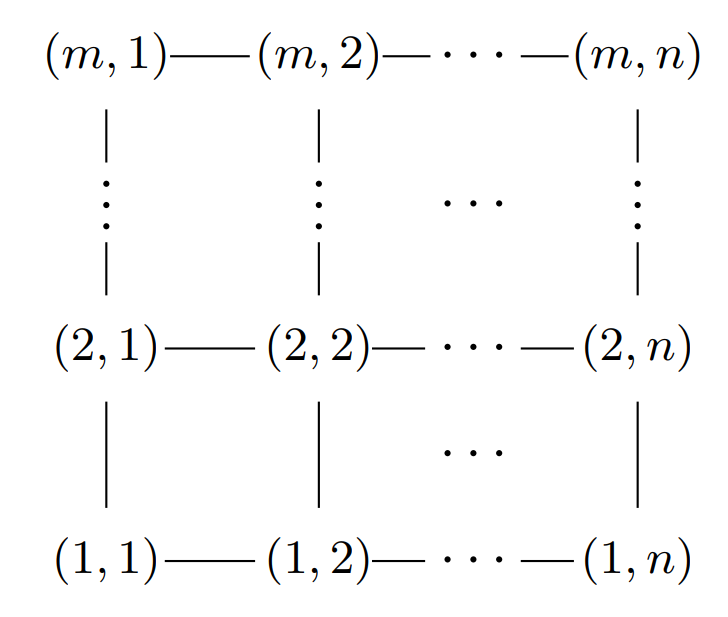
\includegraphics[width=0.2\textwidth]{A4_1.png}
\end{figure}
Your friends want to break into the lucrative coffee shop market by opening a new chain called \textit{The Coffee Pot}. They have a map of the street corners in a neighbourhood of Toronto (shown above), and for each $(i, \; j)$, an estimate $p_{i, \: j} > 0$ of the profit they can make if they open a shop on corner $(i, \; j)$. If they open shops on multiple corners, their profits add up. So ideally, they would like to open a shop at every corner (``the dream").\\
\\
However, if they open a shop on corner $(i, \; j)$, municipal regulations forbid them from opening shops on \textit{adjacent} corners $(i - 1, j)$, $(i + 1, \; j)$, $(i, \; j - 1)$, and $(i, \; j + 1)$ (whichever exist). As you can guess, they would like to select street corners where to open shops in order to maximize their profits!
\begin{enumerate}
    \item[\textbf{(a)}] {[5 Points]} Consider the following greedy algorithm to try and select street corners. Give a precise counter-example to show that this greedy algorithm does not always find an optimal solution. Clearly state your counter-example (values of $m$, $n$, and $p_{i \: j}$ for $1 \leq i \leq m, \; 1 \leq j \leq n)$, the solution found by the greedy algorithm, and a different solution with larger profit.
    \begin{center}
    \begin{algorithmic}[h]
        \State $C \gets \{(i, \; j) : 1 \leq i \leq m, 1 \leq j \leq n\}$  \Comment{$C$ is the set of every available corner}
        \State $S \gets \varnothing$  \Comment{$S$ is the current selection of corners}
        \While {$C \ne \varnothing$}
            \State pick $(i, \; j) \in C$ with the maximum value of $p_{i, \: j}$
            \State \Comment{Add $(i, \; j)$ to the selection and remove it (as well as all corners adjacent to it) from $C$.}
            \State $S \gets S \cup \{(i, \; j)\}$
            \State $C \gets C \setminus \{(i, \; j), \; (i - 1, \; j), \; (i + 1, \; j), \; (i, \; j - 1), \; (i, \; j + 1)\}$
        \EndWhile
        \State \Return $S$
    \end{algorithmic}
    \end{center}
    \begin{mdframed}
        \textit{Solution.}\\ %Q2 a)
        \textbf{Counter-example:}
        \\
        \\Consider this input:
        \[
            \begin{tabular}{c @{\hspace{2\tabcolsep}} *{5}{c}}
            \series 3 & | & 4\\
            \series  \vert&  & \vert\\
            \series 1 & | & 3\\
            \end{tabular}
        \]
        The numbers indicates the profit for each corner:\\
        - $p(1,1) = 3$, $ p(1,2) = 4$, $p(2,1) = 1$, $p(2,2) = 3$\\
        The greedy algorithm in (a) will return $\{(1,2), (2,1)\}$\\
        - profit = $p(1,2) + p(2,1) = 4+1=5$\\
        However the optimal solution is $\{(1,1), (2,2)\}$\\
        - profit = $p(1,1) + p(2,2) = 3 + 3 = 6$\\
        Clearly the optimal solution has larger profit than the solution computed by the greedy algorithm.
        
    \end{mdframed}
    \item[\textbf{(b)}] {[15 Points]} Prove that the greedy algorithm from part (a) gives 4-approximation.\\
    \\
    {[Hint: Let $S$ be the selection returned by the greedy algorithm and
    let $T$ be an optimal solution. Show that for all $(i, \; j) \in T$, either $(i, \; j) \in S$ or there is an adjacent $(i', \; j') \in S$ with $p_{i', \: j'} \geq p_{i, \: j}$. What does this means for all $(i, \; j) \in S$ and their adjacent corners?]}
    \begin{mdframed}
        \textit{Solution.}\\ %Q2 b)
        \textbf{Proof}
        \\For any input $I$,
        \\Let:
        \\- $L(I)$ be the lowest sum of profit
        \\- $U(I)$ be the highest sum of profit
        \\
        \\\textbf{Want to show:} $U(I) \leq 4L(I)$
        \\For any input $I$,
        \\Let:
        \\- $X$ be the output set from the greedy algorithm
        \\- $X_{opt}$ be the set with optimal profit in $I$
        \\
        \\(3) For every $e \in X_{opt}$, if $e \in X_{opt}$ but $e \notin X$, then there must be some $\hat{e} \in X$ such that $p(\hat{e}) \geq p(e)$ and $\hat{e}$ and $e$ are adjacent. Otherwise, $e$ will be added to X based on the implementation of the greedy algorithm.
        \\For every $e \in X$, there are at most 4 distinct adjacent elements, so there are at most 4 elements($e_a \in X_{opt}$, $e_b \in X_{opt}$, $e_c \in X_{opt}$, $e_d \in X_{opt}$) such that $p(e) \geq p(e_a)$ and $p(e) \geq p(e_b)$ and $p(e) \geq p(e_c)$ and $p(e) \geq p(e_d)$ based on (3). So $4p(e) \geq p(e_a)+p(e_b)+p(e_c)+p(e_d)$. In the worst case scenario, $X_{opt}$ contains all such $e_a, e_b, e_c, e_d$, thus, $\sum_{e \in X_{opt}}p(e) \leq 4\sum_{e \in X}p(e)$, and equivalently, $U(I) \leq 4U(I)$.
        
        \\Hence, the greedy algorithm from part (a) gives 4-approximation.
        
    \end{mdframed}
\end{enumerate}

\section*{Q3 [20 Points] Randomized Algorithm}
Recall that a 3CNF formula $\varphi = C_1 \land ... \land C_m$ consists of a conjunction of $m$ clauses, where each clause is a disjunction of \textit{exactly} 3 literals. In the standard (unweighted) Exact Max-3-SAT problem, our goal was to maximize the number of clauses that are ``satisfied" (i.e. in which at least one literal is true). Recall that the naive randomized algorithm from class provides 7/8-approximation for this and can be derandomized.\\
\\
Now, consider a related problem, Exact Robust-Max-3-SAT, in which a clause is considered ``satisfied" when \textit{at least two literals} are true, and the goal is still to maximize the total weight of clauses that are ``satisfied", but under the new definition of clause satisfaction.
\begin{enumerate}
    \item[\textbf{(a)}] {[5 Points]} Give a randomized 1/2-approximation algorithm for Exact Robust-Max-3-SAT. Specifically, your algorithm should return a random truth assignment of variables such that the \textit{expected} number of clauses ``satisfied" is at least $m / 2$. Argue correctness of your algorithm.
    \begin{mdframed}
        \textit{Solution.}\\ %Q3 a)
        \begin{lstlisting}[mathescape=true, numbers=left]
# The input is an array of n variables in the Exact Robust-Max-3-SAT problem.
RamdomlyAssign(vars[1 ... n]):
    # an empty list for returning
    assignedArray = [1 ... n]
    for i = 1 to n:
        Set vars[i] to True or False randomly, each with probability $\frac{1}{2}$
        assignedArray[i] = vars[i]
    return assignedArray
        \end{lstlisting}
    \textbf{\underline{Proof of Correctness:}}
    \begin{proof}
    For each clause $C_i$, $1 \leq i \leq m$:
    \begin{align*}
        Pr[C_i \; is \; satisfied] &= Pr[At \; least \; 2 \; variables \; are \; True]\\
        &= 1 - Pr[At \; most \; 1 \; variable \; is \; True]\\
        &= 1 - Pr[exactly \; no \; variable \; is \; True] - Pr[exactly \; 1 \; variable \; is True]\\
        &= 1 - \frac{1}{2^3} - \frac{3}{2^3}\\
        &= 1 - \frac{1}{8} - \frac{3}{8}\\
        &= \frac{7}{8} - \frac{3}{8}\\
        &= \frac{4}{8}\\
        &= \frac{1}{2}
    \end{align*}
    Let $X$ represents the number of clauses satisfied by the random assignment by this algorithm, then,
    \begin{align*}
        E[X] &= \sum_{i = 1}^{m} 1 \cdot Pr[C_i \; is \; satisfied]\\
        &= \sum_{i = 1}^{m} 1 \cdot \frac{1}{2}\\
        &= \sum_{i = 1}^{m} \frac{1}{2}\\
        &= \frac{m}{2} \geq \frac{OPT}{2}
    \end{align*}
    Thus the algorithm satisfies at least $\frac{m}{2}$ clauses in expect, and this algorithm is a randomized 1/2 - approximation algorithm meets the requirement.
    \end{proof}
    \end{mdframed}
    \item[\textbf{(b)}] {[15 Points]} Derandomize your algorithm to derive a deterministic algorithm which \textit{always} returns a truth assignment of variables ``satisfying" at least $m/2$ clauses. Write pseudocode for your derandomized algorithm, justify its correctness, and analyze its worst-case running time.
    \begin{mdframed}
        \textit{Solution.}\\ %Q3 b)
        To derandomize this problem, an algorithm is needed to maximize the expectation value. The algorithm is listed and a helper algorithm that solves the expectation value is also constructed below. Let $X$ represents the number of clauses satisfied.
\begin{lstlisting}[mathescape=true, numbers=left]
Binomial(unassigned, trueLiteralsNeeded):
    if trueLiteralsNeeded $>$ unassigned:
        return 0
    else:
        # the possibility for either True or False is $\frac{1}{2}$
        # so use $(\frac{1}{2}) ^ {unassigned}$ directly
        # also, this combination computation takes $O(1)$ since
        # unassigned is at most 3 and trueLiteralsNeeded is at most 2
        # which means the upper bound to solve the factorial is constant
        
        return ${unassigned \choose trueLiteralsNeeded} \cdot (\frac{1}{2}) ^ {unassigned}$

ExpectedValue(clauses[1 ... m], assigned{$x_1 ... x_n$},):
    expectedValue = 0
    for clause in clauses:
        # number of literals evaluate to True
        trueCount = 0
        # number of literals evaluate to NIL
        nilCount = 0
        for literal in clauses:
            if assigned[var] is NIL:
                nilCount = nilCount + 1
            else if literal is not negated:
                if assigned[var] is True:
                    trueCount = trueCount + 1
            else if literal is negated:
                if assigned[var] is False:
                    trueCount = trueCount + 1
            
            if $trueCount \geq 2$:
                expectedValue = expectedValue + 1
            # possibility of meeting the clause here respects the
            # binomial distribution about the number unassigned
            # variables and the left number of variables needed to
            # assign true to satisfy the clause
            else expectedValue = expectedValue + Binomial(nilCount, $2 - trueCount$)
    return expectedValue

DeRandomize(vars[1 ... n], clauses[1 ... m]):
    # let assigned be a dictionary mapping each variable
    # to its value, each access to a dictionary takes $O(1)$
    assigned = {}
    # assigned each variable to NIL initially
    for i = 1 to n:
        assigned[$x_i$] = NIL
    for j = 1 to n:
        # actually calling the function ExpectValue, but using
        # mathematical symbol here to increase the readability
        # indeed, the full form is
        # assigned[$x_j$] = True
        # T_sol = ExpectedValue(clauses, assigned)
        # assigned[$x_j$] = False
        # F_sol = ExpectedValue(clauses, assigned)
        T_sol = $E[X|x_1 = assigned[x_1], ..., x_j = True, ..., x_n = assigned[x_n]]$
        F_sol = $E[X|x_1 = assigned[x_1], ..., x_j = False, ..., x_n = assigned[x_n]]$
        if T_sol $\geq$ F_sol:
            assigned[$x_j$] = True
        else assigned[$x_j$] = False
return assigned
\end{lstlisting}
\textbf{\underline{Proof of Correctness:}}
\begin{proof}
In order to derandomize the algorithm, the algorithm should make the expected output more deterministic, therefore, the algorithm \textsc{DeRandomize} returns an assignment that maximizes the expected value. In the algorithm, at first, the algorithm initializes a hash table assigned to store the boolean value assigned to each variable in line 41 and assign each variable to \textsc{Nil} since none of the variable is assigned at this time by the loop in line 43 - 44. Then the algorithm compares the choices of value of $x_i$ ($x_i = True$ or $x_i = False$) and makes the choice leads to a larger expected value with respect to all variables either assigned (i.e., $x_1  \; ... \; x_{i - 1}$) or not assigned (i.e., $x_{i + 1} \; ... \; x_{n}$), each assigned variable has value True or False and unassigned value has the value \textsc{Nil} in lineand all variables from $x_1$ to $x_n$ are checked by the loop specified by the line 45 - 55. Also in each iteration, the choice which gives a higher expected value is finally selected by the line 55 - 57. Therefore, if the algorithm to compute the expected value used in each iteration is correct, then the algorithm \textsc{DeRandomize} is correct.\\
\\
The expectation is computed by the algorithm \textcc{ExpectedValue}. It initialize a counter \textit{expectedValue} equals to 0 at the beginning. For each outer loop, it takes a clause from all clauses in the loop in line 14 and then count for the number of true literal and unassigned literal (i.e., \textit{nilCount}) by the inner loop in line 19 - 27. For each time to sum up the expected value, in the formulae $\sum_{i = 1}^{m}c_i \cdot Pr[c_i \; is \; satisfied]$, $c_i = 1$ since the situation $clause_i$ is satisfied is considered (Otherwise, $c_i = 0$ for the situation $clause_i$ is not satisfied). Therefore, the expected value is the sum of the probability for each clause to get satisfied (i.e., $\sum_{i = 1}^{m}Pr[c_i \; is \; satisfied]$). If there are at least 2 True literals, then the clause is absolutely satisfied (with possibility 1 to satisfy the clause) and the expected value increases by 1. If there are less than 2 True literals, then the expected value increases by the probability that she clause is satisfied. Since the probability is actually ``The probability of `Number of literals being True to satisfy the clause' out of all the unassigned number of variables", which respects to the binomial distribution. Therefore, if the there are more literals to be True in order to satisfy the clause than the actual unassigned variables, then the clause is unsatisfiable, thus the algorithm returns the possibility 0 (not possible to satisfy the clause). Or the algorithm returns the possibility computed by the function \textsc{Binomial}, which is constructed based on the binomial distribution pmf:
\[Bin(n, \; k, \; p) = {n \choose k} \cdot p ^ {k} \cdot (1 - p) ^ {(n - k)}.\]
Therefore, the algorithm can solve the correct amount of possibility to satisfy the clause, thus the expected value increases correctly for each time. Thus, the algorithm \textsc{ExpectedValue} works correctly.\\
\\
In conclusion, since the expected value is solved correctly, then the algorithm \textsc{DeRandomize} has the correct expected value (calculated by the algorithm \textsc{ExpectedValue}) as the clue to make a better choice to maximize the total expected value for each variable. Also, in each iteration of \textsc{DeRandomize}, the total expected value is at least as large as before with the correct choice, then the total expected value after the entire assignment is at least as large as $\frac{m}{2}$, the lower bound of the expected value solved by the na\"ive algorithm \textsc{RandomlyAssign}, therefore, there are at least $\frac{m}{2}$ clauses can be satisfied with the algorithm \textsc{DeRandomized}. 

\end{proof}
\textbf{\underline{Worst-Case Running Time:}}
\begin{itemize}
    \item \textsc{Binomial}:
    \begin{itemize}
        \item line 2 - 3: $O(1)$.
        \item line 4 - 11: $O(1)$
    \end{itemize}
    Thus \textsc{Binomial} takes $O(1)$ in  total.
    \item \textsc{ExpectedValue}:
    \begin{itemize}
        \item line 14: initializing the \textit{expectedValue}: $O(1)$
        \item line 17 - 18: initializing counters: $O(1)$ in total
        \item line 20 - 28: there are fixed number of clausese (3 in total), each access to the hash table takes $O(1)$, and all the comparations and addition take $O(1)$ in total, thus the whole block takes $O(1)$ in total
        \item line 30 - 36: the comparison and addition take $O(1)$, and the algorithm \textsc{Binomial} takes $O(1)$, thus the whole block takes $O(1)$
        \item to sum up, the loop in line 15 - 36 takes $O(1) * O(m) = O(m)$ since there are $m$ clauses input.
    \end{itemize}
    Thus \textsc{ExpectedVaue} takes $O(m) + O(1) = O(m)$ in total.
    \item \textsc{DeRandomize}:
    \begin{itemize}
        \item line 42: construct an empty hash table: $O(1)$
        \item line 44 - 45: initialize the hash map, assign all $n$ variable to \textsc{Nil}: $O(1) * O(n) = O(n)$
        \item line 54 - 55, compute the expected value twice with the opposite assignment to $x_i$, since the algorithm \textsc{ExpectedValue} takes $O(m)$, this block takes $2 * O(m) = O(m)$
        \item line 56 - 58, comparison and the assignment to a variable in the hash table: $O(1)$
        \item line 46 - 58: all blocks in the loop takes $O(m) + O(1) = O(m)$ in total, thus the loop takes $O(n) * O(m) = O(mn)$ in total
    \end{itemize}
    Thus \textsc{DeRandomize} takes $O(mn) + O(n) = O(mn)$ in total. 
\end{itemize}
Therefore, the whole derandomization algorithm takes $O(mn)$ in total for the worst-case complexity.
    \end{mdframed}
\end{enumerate}
\end{document}